% Provenance (never printed): cycle 4 SVT/physique, "La planete Terre,
% l'environnement": the movements of the atmosphere, weather and its
% forecast; see sources/book1/PROVENANCE.md. Book 1, grade 8, chapter 3.
% Vocabulary guard: owns air mass, front (warm, cold), depression (homograph:
% phrase-level linking only), anticyclone, isobar, weather forecast. The
% rotation of the winds around lows and highs is told (deflection, recalled
% from ch. g8.2); the occluded front is named in prose only; numerical models
% are told, not taught.
\chapter{气团、锋与天气图}\label{ch:g8:fronts-and-weather-maps}

清晨\omterm{def:g1:watching-the-weather:weather}{天气}晴朗、风平浪静。正午前后，天空高处出现稀薄的白色条纹，
慢慢铺展成一层淡薄的云幕，遮暗了
太阳。午后\omterm{def:g4:clouds-rain-snow:cloud}{云层}增厚、位置降低；傍晚时
开始下起持续的雨。夜间\omterm{def:g1:watching-the-weather:weather}{天气}转暖、变湿润，随后
一条乌云带带来一阵短促的暴雨和一阵阵风。
次日清晨\omterm{def:g1:watching-the-weather:weather}{天气}晴朗、凉爽且多风。两天之内，一个
\emph{\omterm{def:g8:fronts-and-weather-maps:depression}{低压}}经过小镇，并带着它的两条锋。
% ledger: ucar:warm-front, ucar:cold-front

\begin{omfigure}

\includegraphics[width=0.6\linewidth]{images/book1/ai/g8-rain-arriving.jpg}

 {\small 一幕雨帘在乌云底部笼罩下抵达小镇上空，
而教堂后方仍是晴空（人工智能生成的示意插图，
场景为通用场景）。}
\label{fig:g8:fronts-and-weather-maps:rain}
\end{omfigure}

\omterm{def:g8:fronts-and-weather-maps:forecast}{天气预报}员数日前就已预见到这一变化。本章将说明其原因：
天空中的空气以大团的\omterm{def:g8:fronts-and-weather-maps:air-mass}{气团}形式存在，\omterm{def:g8:fronts-and-weather-maps:air-mass}{气团}沿锋相遇，
而气压图则显示它们的去向。

\begin{recall}
空气对它所接触的一切物体施加压力；气压计测量的正是这种压强，
以百帕为单位（见物理课本），\omterm{def:g4:world-physical-map:altitude}{海平面}附近的气压约为
\qty{1013}{hPa}（见\cref{ch:g8:the-atmosphere}）。湿润空气上升并冷却时形成云，
（见\cref{ch:g4:clouds-rain-snow}）。近地面处，风
从高压吹向\omterm{def:g8:fronts-and-weather-maps:depression}{低压}，而地球自转
使其偏转：在\omterm{def:g3:continents-and-oceans:equator}{北半球}向右偏。大约在
\ang{30} 与 \ang{60} 之间，\omterm{def:g8:winds-global-circulation:global-winds}{西风带}带来接连不断的\omterm{def:g5:natural-hazards:storm}{风暴}
（见\cref{ch:g8:winds-global-circulation}）。
\end{recall}

\section{气团}

在同一地点停留数日的空气，会获得
其下方地表的性质：在温暖的洋面上空，它变得温暖湿润；在
冰冻的陆地上空，它变得寒冷干燥。当它离开时，便将这种性质
带走，有时可远行数千千米。
% ledger: noaa:air-mass

\begin{definition}[气团]\label{def:g8:fronts-and-weather-maps:air-mass}
称\emph{气团}\index{气团}为一大团空气，其中
在给定高度上，各处的温度与湿度
基本相同。它的这些性质取自其形成的区域，即其
\emph{源地}。
\end{definition}
% ledger: noaa:air-mass

预报员用两个字母为\omterm{def:g8:fronts-and-weather-maps:air-mass}{气团}命名。第一个字母表示其形成地：
\emph{c}（\omterm{def:g3:continents-and-oceans:continent}{大陆}性）表示形成于陆地上空，因此干燥；\emph{m}
（\omterm{def:g2:water-on-earth:ocean}{海洋}性）表示形成于\omterm{def:g2:water-on-earth:ocean}{海洋}上空，因此湿润。第二个字母表示其冷暖程度：
\emph{A}（\omterm{def:g3:continents-and-oceans:poles}{北极}性）表示形成于极地上空，\emph{P}（极地性）表示形成于
高\omterm{def:g6:latitude-longitude:latitude}{纬度}地区，\emph{T}（热带性）表示形成于低\omterm{def:g6:latitude-longitude:latitude}{纬度}地区。来自
炎热\omterm{def:g5:weather-and-climate:desert}{沙漠}的空气为 cT，炎热干燥；来自\omterm{def:g3:continents-and-oceans:poles}{北极}的空气为 cA，极其寒冷且
干燥。
% ledger: noaa:air-mass

\begin{omfigure}
\begin{tikzpicture}
\begin{axis}[ommap, width=12.6cm, xmin=-100, xmax=60, ymin=10, ymax=85,
  xtick={-90,-60,...,60}, ytick={20,40,60,80},
  xticklabels={$90^\circ$西, $60^\circ$西, $30^\circ$西, $0^\circ$,$30^\circ$东, $60^\circ$东},
  yticklabels={$20^\circ$北, $40^\circ$北, $60^\circ$北, $80^\circ$北},
  tick label style={font=\scriptsize}]
  \addplot[fill=omLithAlluv, draw=black!45, line width=0.2pt] table {figdata/out/shared-geo-land.dat};
  \tikzset{src/.style={line width=0.9pt, fill opacity=0.35, text opacity=1, font=\scriptsize, align=center}}
  \draw[src, draw=omCold, fill=omCold!35] (axis cs:-30,79) ellipse [x radius=26, y radius=4.5];
  \node[font=\scriptsize, align=center, fill=white, inner sep=1pt] at (axis cs:-30,79) {\textbf{cA}：极寒、干燥};
  \draw[src, draw=omCold, fill=omCold!25] (axis cs:-35,55) ellipse [x radius=14, y radius=6];
  \node[font=\scriptsize, align=center, fill=white, inner sep=1pt] at (axis cs:-35,55) {\textbf{mP}：寒冷、\\湿润};
  \draw[src, draw=omCold, fill=omCold!25] (axis cs:-84,60) ellipse [x radius=12, y radius=7];
  \node[font=\scriptsize, align=center, fill=white, inner sep=1pt] at (axis cs:-84,60) {\textbf{cP}：寒冷、\\干燥};
  \draw[src, draw=omCold, fill=omCold!25] (axis cs:45,62) ellipse [x radius=14, y radius=7];
  \node[font=\scriptsize, align=center, fill=white, inner sep=1pt] at (axis cs:45,62) {\textbf{cP}：寒冷、\\干燥};
  \draw[src, draw=omWarm, fill=omWarm!25] (axis cs:-45,28) ellipse [x radius=16, y radius=6];
  \node[font=\scriptsize, align=center, fill=white, inner sep=1pt] at (axis cs:-45,28) {\textbf{mT}：温暖、\\湿润};
  \draw[src, draw=omWarm, fill=omWarm!25] (axis cs:10,24) ellipse [x radius=15, y radius=6];
  \node[font=\scriptsize, align=center, fill=white, inner sep=1pt] at (axis cs:10,24) {\textbf{cT}：炎热、\\干燥};
\end{axis}
\end{tikzpicture}

{\small 北大西洋周围\omterm{def:g8:fronts-and-weather-maps:air-mass}{气团}的典型源地
（示意）：\omterm{def:g3:continents-and-oceans:poles}{北极}上空、寒冷的\omterm{def:g3:continents-and-oceans:continent}{大陆}、北方\omterm{def:g2:water-on-earth:ocean}{海洋}、
亚热带\omterm{def:g2:water-on-earth:ocean}{海洋}和撒哈拉\omterm{def:g5:weather-and-climate:desert}{沙漠}。蓝色为冷\omterm{def:g8:fronts-and-weather-maps:air-mass}{气团}，红色为暖\omterm{def:g8:fronts-and-weather-maps:air-mass}{气团}。}
% ledger: noaa:air-mass, data:ne-land (schematic regions)
\label{fig:g8:fronts-and-weather-maps:sources}
\end{omfigure}

\section{锋}

当一个\omterm{def:g8:fronts-and-weather-maps:air-mass}{气团}移动时，它会与另一个\omterm{def:g8:fronts-and-weather-maps:air-mass}{气团}相遇。两者不易混合：
它们保持分离，二者之间有一条狭窄的边界，
\omterm{def:g1:watching-the-weather:weather}{天气}在此发生变化。
% ledger: mo:fronts, ucar:cold-front

\begin{definition}[锋]\label{def:g8:fronts-and-weather-maps:front}
称\emph{锋}\index{锋}为地面上两个温度与湿度不同的\omterm{def:g8:fronts-and-weather-maps:air-mass}{气团}之间的
边界。在\emph{冷
锋}\index{冷锋}处，冷空气推入较暖的空气，
并取代其位置；在\emph{暖锋}\index{暖锋}处，暖空气推入
较冷的空气，并取代其位置。
\end{definition}
% ledger: mo:fronts, ucar:cold-front, ucar:warm-front

冷空气比暖空气密度大。在\omterm{def:g8:fronts-and-weather-maps:front}{冷锋}处，冷空气
像楔子一样滑到暖空气下方，并把暖空气急剧抬升。温暖潮湿的空气
迅速上升，形成高耸的\omterm{def:g4:clouds-rain-snow:cloud-families}{积云}和\omterm{def:g4:clouds-rain-snow:cloud-families}{积雨云}：锋面
带来强\omterm{def:g4:clouds-rain-snow:precipitation}{降水}，有时伴有\omterm{def:g4:clouds-rain-snow:precipitation}{冰雹}和雷暴、阵风以及
气温骤降。锋面过境后，雨停，天空
放晴。\omterm{def:g8:fronts-and-weather-maps:front}{冷锋}移动很快，可达\omterm{def:g8:fronts-and-weather-maps:front}{暖锋}速度的两倍。
% ledger: ucar:cold-front

\begin{omfigure}
\begin{tikzpicture}[font=\footnotesize, >={Stealth[length=2.2mm]}, yscale=0.7, xscale=0.95]
  % ground
  \draw[line width=0.8pt] (0,0) -- (15,0);
  % cold wedge, nose at x = 8.2
  \fill[omCold!18] (0,0) -- (0,3.4) .. controls (4.5,3.2) and (7.2,2.4) .. (7.9,0.8)
    .. controls (8.1,0.35) and (8.2,0.12) .. (8.25,0) -- cycle;
  \draw[omCold, line width=1pt] (0,3.4) .. controls (4.5,3.2) and (7.2,2.4) .. (7.9,0.8)
    .. controls (8.1,0.35) and (8.2,0.12) .. (8.25,0);
  \node[omCold, align=center] at (3.2,1.4) {\textbf{冷空气}\\（密度大）};
  \node[omWarm, align=center] at (12.6,1.4) {\textbf{暖湿空气}};
  % cold air pushes
  \draw[->, omCold, line width=1.2pt] (4.6,0.5) -- (7.0,0.5);
  % warm air lifted
  \draw[->, omWarm, line width=1.2pt] (11.2,0.45) .. controls (9.4,0.6) and (8.6,1.4) .. (8.5,3.0);
  % cumulonimbus
  \fill[black!12] (7.3,2.6) .. controls (7.0,3.4) and (7.4,4.2) .. (7.9,4.5)
    .. controls (7.6,5.0) and (8.6,5.2) .. (9.4,5.1) -- (11.0,5.15)
    .. controls (10.6,4.9) and (10.2,4.8) .. (10.0,4.6)
    .. controls (10.4,4.0) and (10.2,3.0) .. (9.8,2.5) -- cycle;
  \draw[black!45] (7.3,2.6) .. controls (7.0,3.4) and (7.4,4.2) .. (7.9,4.5)
    .. controls (7.6,5.0) and (8.6,5.2) .. (9.4,5.1) -- (11.0,5.15)
    .. controls (10.6,4.9) and (10.2,4.8) .. (10.0,4.6)
    .. controls (10.4,4.0) and (10.2,3.0) .. (9.8,2.5) -- cycle;
  \node at (9.0,3.8) {积雨云};
  \foreach \x in {7.7,8.0,...,9.6} \draw[omCold!70, line width=0.5pt] (\x,2.45) -- (\x-0.25,0.15);
  \node[anchor=west, align=left] at (9.8,1.95) {强降水，\\阵风};
  % motion
  \draw[->, line width=1.3pt] (5.7,4.3) -- (7.2,4.3);
  \node[anchor=east] at (5.6,4.3) {锋面移动方向};
  \node[anchor=north] at (8.25,-0.1) {地面锋面};
  \node[anchor=north west, align=left] at (0.1,-0.1) {锋后：较凉，天气转晴};
  \node[anchor=north east, align=right] at (15,-0.1) {锋前：温暖潮湿};
\end{tikzpicture}

{\small 从侧面看到的\omterm{def:g8:fronts-and-weather-maps:front}{冷锋}（高度做了大幅夸张）。冷空气
像楔子一样插到暖空气下方，暖空气被陡然抬升，
形成高耸的云。}
% ledger: ucar:cold-front
\label{fig:g8:fronts-and-weather-maps:cold}
\end{omfigure}

在\omterm{def:g8:fronts-and-weather-maps:front}{暖锋}处，轻而暖的空气无法把冷空气推离地面：
它沿着一个长而平缓的斜坡慢慢爬升到冷空气之上。它的
云因此远在锋面之前、高挂天空中出现：
先是细丝状的\omterm{def:g4:clouds-rain-snow:cloud-families}{卷云}，然后是卷\omterm{def:g4:clouds-rain-snow:cloud-families}{层云}形成的薄纱，再是灰色的高\omterm{def:g4:clouds-rain-snow:cloud-families}{层云}。
随着锋面靠近，\omterm{def:g4:clouds-rain-snow:cloud}{云层}变得更低、更厚，
一场长时间、持续而均匀的降雨随之开始。锋面过境后，空气变得更暖、更
潮湿。
% ledger: ucar:warm-front, bom:isobars (warm front: steady rain, grey skies)

\begin{omfigure}
\begin{tikzpicture}[font=\footnotesize, >={Stealth[length=2.2mm]}]
  \draw[line width=0.8pt] (0,0) -- (15,0);
  % cold air ahead (right), warm air climbing a gentle slope from the front at x = 2.2
  \fill[omCold!18] (2.2,0) .. controls (6,0.9) and (10,2.2) .. (15,3.4) -- (15,0) -- cycle;
  \draw[omCold, line width=1pt] (2.2,0) .. controls (6,0.9) and (10,2.2) .. (15,3.4);
  \node[omCold, align=center] at (11.8,0.75) {\textbf{冷空气}};
  \node[omWarm, align=center] at (1.4,1.6) {\textbf{暖湿}\\\textbf{空气}};
  \draw[->, omWarm, line width=1.2pt] (1.0,0.45) .. controls (4.5,0.9) and (8.5,2.4) .. (12.4,3.4);
  % clouds: nimbostratus near the front, altostratus, cirrostratus, cirrus far ahead
  \fill[black!18] (2.4,0.7) .. controls (3.2,1.8) and (5.5,2.3) .. (6.6,2.4) -- (6.4,1.25) .. controls (5,1.0) and (3.8,0.7) .. cycle;
  \node at (5.4,1.62) {雨层云};
  \foreach \x in {3.0,3.3,...,5.7} \draw[omCold!70, line width=0.5pt] (\x,0.95) -- (\x-0.2,0.25);
  \fill[black!10, rounded corners=4pt] (6.4,2.65) rectangle (10.0,3.25);
  \node at (8.2,2.95) {高层云};
  \fill[black!6, rounded corners=4pt] (9.6,3.75) rectangle (12.6,4.15);
  \node at (11.1,3.95) {卷层云};
  \foreach \x in {12.6,13.2,13.8} \draw[black!35, line width=0.6pt] (\x,4.55) .. controls (\x+0.2,4.75) and (\x+0.4,4.6) .. (\x+0.55,4.85);
  \node[anchor=south] at (13.4,4.9) {卷云};
  \draw[->, line width=1.3pt] (2.6,4.3) -- (4.1,4.3);
  \node[anchor=east] at (2.5,4.3) {锋面移动方向};
  \node[anchor=north] at (2.2,-0.1) {地面锋面};
  \node[anchor=north east] at (15,-0.1) {锋前远处：最早出现的高云};
\end{tikzpicture}

{\small 从侧面看到的\omterm{def:g8:fronts-and-weather-maps:front}{暖锋}（高度做了大幅夸张）。暖空气
缓慢爬升到冷空气之上；随着锋面靠近，\omterm{def:g4:clouds-rain-snow:cloud}{云层}变得更低、更厚，
降雨长时间而均匀。}
% ledger: ucar:warm-front
\label{fig:g8:fronts-and-weather-maps:warm}
\end{omfigure}

在\omterm{def:g1:watching-the-weather:weather-chart}{天气图}上，\omterm{def:g8:fronts-and-weather-maps:front}{冷锋}用带三角形的蓝线表示，\omterm{def:g8:fronts-and-weather-maps:front}{暖
锋}用带半圆的红线表示。符号画在锋面
移动方向的一侧。当快速移动的\omterm{def:g8:fronts-and-weather-maps:front}{冷锋}赶上\omterm{def:g8:fronts-and-weather-maps:front}{暖锋}时，
两者合并成\emph{锢囚锋}，以紫色线表示，
并同时标注两种符号。
% ledger: mo:fronts, ucar:cold-front

\section{低压与高压}

锋面诞生于穿越中\omterm{def:g6:latitude-longitude:latitude}{纬度}地区的大型气旋
之中。空气上升处，地面气压低于四周；
空气下沉处，气压则高于四周。
% ledger: bom:highs-lows

\begin{definition}[低压与高压]\label{def:g8:fronts-and-weather-maps:depression}
称\emph{低压}\index{低压（天气）}，或低气压，为
\omterm{def:g4:world-physical-map:altitude}{海平面}气压低于周围所有地区的区域。
称\emph{反气旋}\index{反气旋}，或高压，为\omterm{def:g4:world-physical-map:altitude}{海平面}气压
高于周围所有地区的区域。
\end{definition}
% ledger: bom:isobars, bom:highs-lows
\phantomsection\label{def:g8:fronts-and-weather-maps:anticyclone}

风由高压吹向\omterm{def:g8:fronts-and-weather-maps:depression}{低压}，但地球自转使其偏转，
因而风几乎绕着中心吹动。在\omterm{def:g3:continents-and-oceans:equator}{北半球}，
风绕\omterm{def:g8:fronts-and-weather-maps:depression}{低压}呈逆时针旋转，
绕\omterm{def:g8:fronts-and-weather-maps:depression}{反气旋}呈顺时针旋转；在\omterm{def:g3:continents-and-oceans:equator}{南半球}则方向相反。
在\omterm{def:g8:fronts-and-weather-maps:depression}{低压}中，近地面的空气向内流动，
上升、冷却并形成云：\omterm{def:g8:fronts-and-weather-maps:depression}{低压}带来云、雨、风及其锋面。
在\omterm{def:g8:fronts-and-weather-maps:depression}{反气旋}中，空气下沉，下降时变暖：
\omterm{def:g8:fronts-and-weather-maps:depression}{反气旋}带来干燥、稳定的\omterm{def:g1:watching-the-weather:weather}{天气}，风力较弱。
典型\omterm{def:g8:fronts-and-weather-maps:depression}{反气旋}中心的气压约为 \qty{1020}{hPa} 或更高；
深厚\omterm{def:g8:fronts-and-weather-maps:depression}{低压}的气压则低于 \qty{980}{hPa}。
% ledger: bom:highs-lows, bom:isobars, mo:global-circ

\begin{omfigure}
\begin{minipage}[c]{0.36\linewidth}\centering
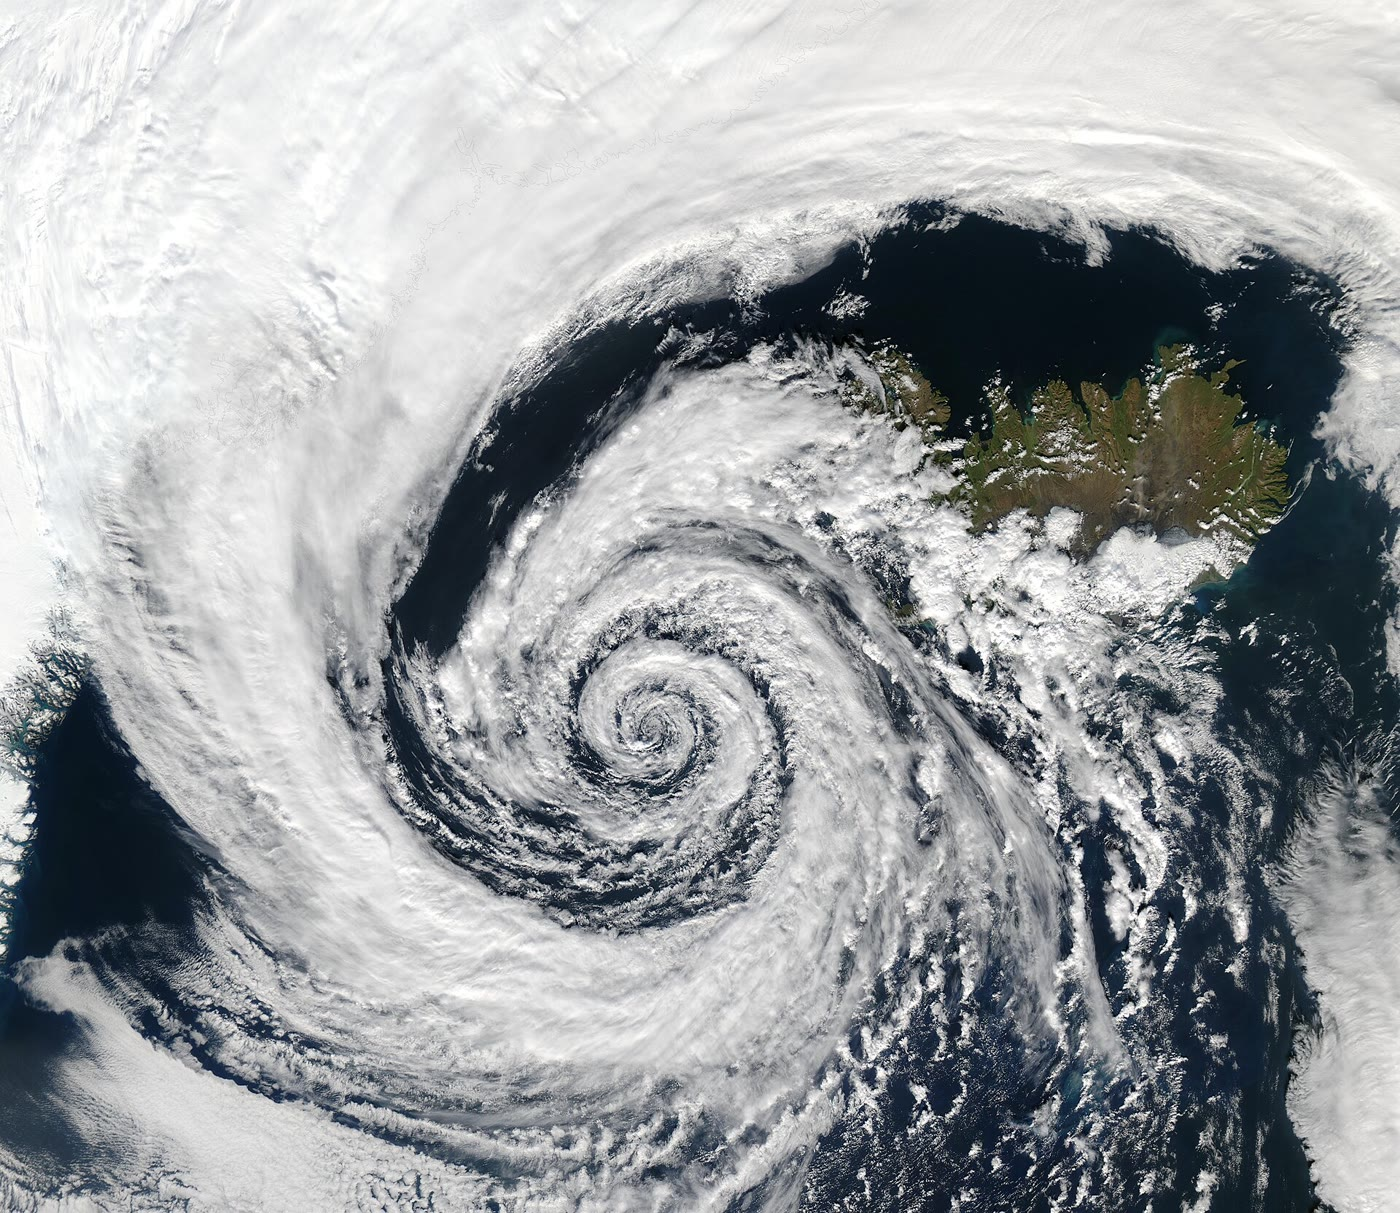
\includegraphics[width=\linewidth]{images/book1/g8-iceland-low.jpg}
\end{minipage}\hfill
\begin{minipage}[c]{0.6\linewidth}\raggedright
{\small 冰岛西南方的\omterm{def:g8:fronts-and-weather-maps:depression}{低压}（冰岛位于右上角），
由 NASA 的 Aqua 卫星于 2003 年 9 月 4 日拍摄。其\omterm{def:g4:clouds-rain-snow:cloud}{云团}螺旋
向中心汇聚，并呈逆时针旋转，
与\omterm{def:g3:continents-and-oceans:equator}{北半球}所有\omterm{def:g8:fronts-and-weather-maps:depression}{低压}相同。NASA/GSFC, MODIS Rapid Response Team, Jacques
Descloitres（公有领域，经由维基共享资源）。}
\end{minipage}
% ledger: commons:iceland-low, bom:highs-lows
\label{fig:g8:fronts-and-weather-maps:iceland}
\end{omfigure}

\section{等压线与天气图}

为了观察\omterm{def:g8:fronts-and-weather-maps:depression}{低压}和\omterm{def:g8:fronts-and-weather-maps:depression}{反气旋}，预报员会绘制气压图。
每个测站都测量本站气压，并将其换算到\omterm{def:g4:world-physical-map:altitude}{海平面}，
以便将山上的测站与\omterm{def:g1:landscapes-around-us:water}{海岸}上的测站相比较。
然后，画出穿过所有气压相同地点的线，
即\omterm{def:g8:fronts-and-weather-maps:isobar}{等压线}。
% ledger: bom:isobars

\begin{definition}[等压线]\label{def:g8:fronts-and-weather-maps:isobar}
称\emph{等压线}\index{等压线}为\omterm{def:g2:drawing-to-map:map}{地图}上连接\omterm{def:g4:world-physical-map:altitude}{海平面}气压
相同地点的线。等压线以百帕为单位标注，
通常每隔 \qty{4}{hPa} 绘制一条。
\end{definition}
% ledger: bom:isobars (the 4 hPa step is the one of this book's maps)

在\omterm{def:g8:fronts-and-weather-maps:depression}{低压}周围，\omterm{def:g8:fronts-and-weather-maps:isobar}{等压线}形成闭合环线，中心气压最低，
标记为 L；在\omterm{def:g8:fronts-and-weather-maps:depression}{反气旋}周围，\omterm{def:g8:fronts-and-weather-maps:isobar}{等压线}同样形成闭合环线，
中心气压最高，标记为 H。\omterm{def:g8:fronts-and-weather-maps:isobar}{等压线}密集处，
气压在相邻地点之间变化越快，风力也越强；
\omterm{def:g8:fronts-and-weather-maps:isobar}{等压线}稀疏之处，风力则较弱。
% ledger: bom:isobars

\begin{omfigure}
\begin{tikzpicture}
\begin{axis}[width=14cm, axis equal image, xmin=0, xmax=2400, ymin=0, ymax=1600,
  hide axis, clip=true, axis background/.style={fill=white}]
  \addplot[isobar] table {figdata/out/grade-8-weather_map-isobars.dat};
  \addplot[warm front] table {figdata/out/grade-8-weather_map-warm.dat};
  \addplot[cold front] table {figdata/out/grade-8-weather_map-cold.dat};
  \addplot[quiver={u=\thisrow{u}, v=\thisrow{v}}, -{Stealth[length=1.5mm]}, omMeth, line width=0.6pt]
    table[x=x, y=y] {figdata/out/grade-8-weather_map-winds.dat};
  \addplot[only marks, mark=none, nodes near coords, point meta=explicit symbolic,
    every node near coord/.style={anchor=center, font=\tiny, fill=white, inner sep=0.6pt}]
    table[x=x, y=y, meta=level] {figdata/out/grade-8-weather_map-labels.dat};
  \node[font=\Large\bfseries, omCold, fill=white, inner sep=1pt] at (axis cs:690,1010) {L};
  \node[font=\scriptsize, anchor=north, fill=white, inner sep=0.5pt] at (axis cs:690,968) {980};
  \node[font=\Large\bfseries, omWarm] at (axis cs:1950,520) {H};
  \node[font=\scriptsize, anchor=north] at (axis cs:1950,485) {1034};
  \addplot[only marks, mark=square*, mark size=2pt, black] table[x=x, y=y] {figdata/out/grade-8-weather_map-town.dat};
  \node[font=\footnotesize\bfseries, anchor=west, fill=white, inner sep=1pt] at (axis cs:870,380) {T};
  \fill[white] (axis cs:1930,1450) rectangle (axis cs:2290,1585);
  \draw[line width=1pt] (axis cs:1950,1480) -- (axis cs:2250,1480);
  \pgfplotsinvokeforeach{1950,2050,2150,2250}{\draw (axis cs:#1,1460) -- (axis cs:#1,1500);}
  \node[font=\scriptsize, anchor=south] at (axis cs:2100,1495) {300 千米};
\end{axis}
\end{tikzpicture}

{\small \omterm{def:g3:continents-and-oceans:equator}{北半球}某个假想日的\omterm{def:g1:watching-the-weather:weather-chart}{天气图}，
由气压模型计算得出。\omterm{def:g8:fronts-and-weather-maps:isobar}{等压线}每隔 \qty{4}{hPa} 绘制一条；
\omterm{def:g8:fronts-and-weather-maps:depression}{低压} L（\qty{980}{hPa}）带有一条\omterm{def:g8:fronts-and-weather-maps:front}{暖锋}（红色）和一条\omterm{def:g8:fronts-and-weather-maps:front}{冷锋}
（蓝色）；\omterm{def:g8:fronts-and-weather-maps:depression}{反气旋} H（\qty{1034}{hPa}）位于东侧。绿色箭头：
表示风，风越强箭头越长。T：本题所指的城镇。}
% ledger: bom:isobars, bom:highs-lows, mo:fronts (figdata/grade-8/weather_map.py)
\label{fig:g8:fronts-and-weather-maps:map}
\end{omfigure}

\begin{method}[读懂天气图]
\begin{enumerate}
  \item 找出中心：\omterm{def:g8:fronts-and-weather-maps:depression}{低压}记为 L，\omterm{def:g8:fronts-and-weather-maps:depression}{反气旋}记为 H，
        并读出它们的气压。
  \item 读取\omterm{def:g8:fronts-and-weather-maps:isobar}{等压线}：数值朝 H 方向升高，朝 L 方向降低。
        \omterm{def:g8:fronts-and-weather-maps:isobar}{等压线}密集意味着风力较强。
  \item 判断风向：\omterm{def:g3:continents-and-oceans:equator}{北半球}的风几乎沿\omterm{def:g8:fronts-and-weather-maps:isobar}{等压线}吹动，
        \omterm{def:g8:fronts-and-weather-maps:depression}{低压}位于风的左侧，
        并略向\omterm{def:g8:fronts-and-weather-maps:depression}{低压}一侧偏转。
  \item 找出锋面及其移动方向（以其符号所在的一侧为准），
        再看两侧的空气：接下来会来什么样的空气？
\end{enumerate}
\end{method}
% ledger: bom:isobars, bom:highs-lows, mo:fronts

\begin{example}[城镇 T 的天气]
图中，T 位于\omterm{def:g8:fronts-and-weather-maps:front}{暖锋}以南、\omterm{def:g8:fronts-and-weather-maps:front}{冷锋}以东，
即两锋之间的暖\omterm{def:g8:fronts-and-weather-maps:air-mass}{气团}中。\omterm{def:g8:fronts-and-weather-maps:front}{暖锋}已经
经过该地。此处\omterm{def:g8:fronts-and-weather-maps:isobar}{等压线}自西南走向东北，\omterm{def:g8:fronts-and-weather-maps:depression}{低压}位于西北，
因此风从西南吹来，温暖而湿润。
\omterm{def:g8:fronts-and-weather-maps:front}{冷锋}自西而来，其三角形标记朝东，
指向该城镇：数小时内将出现一阵短暂的强\omterm{def:g4:clouds-rain-snow:precipitation}{降水}和阵风，
随后风向转为西风或西北风，
空气变凉，天空转晴。
\end{example}
% ledger: ucar:cold-front (figdata/grade-8/weather_map.py: wind at T from 227 degrees)

气压计即使没有\omterm{def:g1:watching-the-weather:weather-chart}{天气图}，也能自己发出预警。设想上图的整张\omterm{def:g1:watching-the-weather:weather-chart}{天气图}
形状不变地以每小时 \qty{40}{km} 的速度向东平移，
并设在锋面以东的站点 S 处有一台自记气压计。两天
半内，它将描出下面的记录。

\begin{omfigure}
\begin{tikzpicture}
\begin{axis}[width=0.86\linewidth, height=5.4cm, xmin=0, xmax=60, ymin=980, ymax=1040,
  xtick={0,12,...,60}, ytick={980,990,...,1040},
  xlabel={记录开始后的小时数}, ylabel={气压 (hPa)},
  axis x line=bottom, axis y line=left, axis line style={-},
  grid=major, grid style={black!10},
  tick label style={font=\scriptsize}, label style={font=\small}, clip=false]
  \draw[omWarm!80!black, dashed] (axis cs:26.28,980) -- (axis cs:26.28,1040);
  \draw[omCold!80!black, dashed] (axis cs:38.49,980) -- (axis cs:38.49,1040);
  \node[font=\scriptsize, omWarm!80!black, anchor=south, fill=white, inner sep=1pt] at (axis cs:26.28,1032) {暖锋};
  \node[font=\scriptsize, omCold!80!black, anchor=south, fill=white, inner sep=1pt] at (axis cs:38.49,1032) {冷锋};
  \addplot[black!80, line width=1pt] table[x=hour, y=p_hPa] {figdata/out/grade-8-barogram-trace.dat};
  \node[font=\scriptsize, anchor=north west, align=left] at (axis cs:2,1028) {反气旋：\\天气稳定};
  \node[font=\scriptsize, anchor=west] at (axis cs:39.5,986) {最低};
\end{axis}
\end{tikzpicture}

{\small 站点 S 处气压计的记录，其间上图所示\omterm{def:g1:watching-the-weather:weather-chart}{天气图}
以每小时 \qty{40}{km} 的速度向东平移（虚构情形，
依据\omterm{def:g1:watching-the-weather:weather-chart}{天气图}的气压场算出）。虚线表示\omterm{def:g8:fronts-and-weather-maps:front}{暖锋}与\omterm{def:g8:fronts-and-weather-maps:front}{冷锋}
经过该站的时刻。}
% ledger: (invented region: weather situation of figdata/grade-8/weather_map.py, record from figdata/grade-8/barogram.py)
\end{omfigure}

\begin{example}[读懂气压计的记录]\label{ex:g8:fronts-and-weather-maps:barogram}
前 8 小时内，气压升至约 \qty{1031}{hPa}，
\omterm{def:g8:fronts-and-weather-maps:depression}{反气旋}经过 S 站，\omterm{def:g1:watching-the-weather:weather}{天气}稳定。此后气压持续下降 30
小时，下降约 \qty{45}{hPa}，\omterm{def:g8:fronts-and-weather-maps:depression}{低压}正在靠近。气压在\omterm{def:g8:fronts-and-weather-maps:front}{暖锋}过境前几小时下降最快，
随后在暖\omterm{def:g8:fronts-and-weather-maps:air-mass}{气团}中下降较慢，
并在\omterm{def:g8:fronts-and-weather-maps:front}{冷锋}过境时降至最低，约 \qty{986}{hPa}，
此后气压回升，\omterm{def:g8:fronts-and-weather-maps:depression}{低压}远去，\omterm{def:g8:fronts-and-weather-maps:front}{冷锋}之后
较凉、较清朗的空气到达。
% ledger: (invented region: figdata/grade-8/barogram.py), bom:highs-lows
\end{example}

\section{天气预报是如何做出的}

\begin{definition}[天气预报]\label{def:g8:fronts-and-weather-maps:forecast}
称\emph{天气预报}\index{天气预报}为对某地未来数小时或数天内
预期\omterm{def:g1:watching-the-weather:weather}{天气}的陈述，
它依据对大气的观察结果及物理定律得出。
\end{definition}
% ledger: mo:how-forecasts

\omterm{def:g8:fronts-and-weather-maps:forecast}{天气预报}分三步做出。第一，全球各地的气象服务机构
每天进行数以百万计的观察：温度、\omterm{def:g4:clouds-rain-snow:precipitation}{降水}量、
气压、风和湿度，测量手段包括地面站、海上、
气象探空气球、雷达和卫星。随后，这些观察结果
被输入计算机模型：功能强大的计算机逐步推算
大气从现状出发将如何变化。最后，预报员
读取结果，并将其与本地区的已知情况相比较，
撰写预报。
% ledger: mo:how-forecasts

\begin{history}[首次公开发布的天气预报]
1854 年，海军军官罗伯特·菲茨罗伊被任命为伦敦新设
气象局的负责人。每天上午 9 点，\omterm{def:g1:landscapes-around-us:water}{海岸}各站测量\omterm{def:g1:watching-the-weather:weather}{天气}，
并用电报把读数发往伦敦；电报是当时最新的发明。
1859 年，一场猛烈的\omterm{def:g5:natural-hazards:storm}{风暴}，
“皇家宪章号”大\omterm{def:g5:natural-hazards:storm}{风暴}击沉了许多船只，菲茨罗伊随后
为水手设立了\omterm{def:g5:natural-hazards:storm}{风暴}预警服务，该服务于 1861 年 2 月开始。
1861 年 8 月 1 日，他更进一步，在报纸上公开发布了
首份面向公众的\omterm{def:g8:fronts-and-weather-maps:forecast}{天气预报}，刊登在《泰晤士报》上。他的预报
只能展望未来一两天，且十分笼统，它们是我们今天
所读预报的开端。
\end{history}
% ledger: mo:fitzroy

\omterm{def:g8:fronts-and-weather-maps:forecast}{天气预报}已大有进步。过去几十年间，预报员
大约每十年多获得一天的有效预报：
如今提前四天的预报，其可靠程度相当于三十年前提前一天的预报。
但预报展望得越远，
可靠性就越低，因为最初观察结果中的微小误差，
会随着计算机向前推算时间而逐步放大。
% ledger: bauer:day-per-decade, mo:accuracy

\begin{inthefield}[观察锋面的到来]
在预报宣布有锋面过境的日子里，每隔几小时看一次天空，记下
时间、云、风和温度。
\omterm{def:g8:fronts-and-weather-maps:front}{暖锋}来临前，是否先出现高空\omterm{def:g4:clouds-rain-snow:cloud-families}{卷云}条纹？\omterm{def:g8:fronts-and-weather-maps:front}{冷锋}过境时，
温度是否下降，风向是否改变？请将你的记录
与当天的\omterm{def:g1:watching-the-weather:weather-chart}{天气图}相比较。
\end{inthefield}

\section{练习}

\begin{exercise}[$\star$]\label{exo:g8:fronts-and-weather-maps:1}
说明下列每对字母的含义，并判断该\omterm{def:g8:fronts-and-weather-maps:air-mass}{气团}是
暖的还是冷的、潮湿的还是干燥的：(a) mT；(b) cP；(c) cT；(d) mP。
\end{exercise}

\begin{exercise}[$\star$]\label{exo:g8:fronts-and-weather-maps:2}
将\omterm{def:g1:watching-the-weather:weather-chart}{天气图}上的每个符号与其含义配对：蓝线加三角形；
红线加半圆；连接气压相同各地的线；
字母 H；字母 L。
\end{exercise}

\begin{exercise}[$\star$]\label{exo:g8:fronts-and-weather-maps:3}
判断下列陈述是否正确，并改正错误的句子。(a) \omterm{def:g8:fronts-and-weather-maps:depression}{反气旋}通常带来
\omterm{def:g1:watching-the-weather:weather}{天气}稳定。(b) \omterm{def:g8:fronts-and-weather-maps:front}{暖锋}的云系在锋面过境后才到达。
(c) \omterm{def:g8:fronts-and-weather-maps:isobar}{等压线}密集意味着风较弱。(d) 冷空气
比暖空气的密度大。
\end{exercise}

\begin{exercise}[$\star$]\label{exo:g8:fronts-and-weather-maps:4}
在本章的\omterm{def:g1:watching-the-weather:weather-chart}{天气图}上：(a) \omterm{def:g8:fronts-and-weather-maps:depression}{低压}中心的
气压是多少？(b) \omterm{def:g8:fronts-and-weather-maps:depression}{反气旋}中心的气压是多少？(c) 相邻两条
\omterm{def:g8:fronts-and-weather-maps:isobar}{等压线}之间相差多少百帕？(d) 两个中心的气压
相差多少百帕？
\end{exercise}

\begin{exercise}[$\star\star$]\label{exo:g8:fronts-and-weather-maps:5}
将下列事件按\omterm{def:g8:fronts-and-weather-maps:front}{暖锋}接近并经过时
的发生先后次序排列：持续性降雨；细条状\omterm{def:g4:clouds-rain-snow:cloud-families}{卷云}；灰色的
高\omterm{def:g4:clouds-rain-snow:cloud-families}{层云}幕；变暖、变湿的空气；\omterm{def:g4:clouds-rain-snow:cloud}{云层}变得更低、更厚。
\end{exercise}

\begin{exercise}[$\star\star$]\label{exo:g8:fronts-and-weather-maps:6}
解释为什么\omterm{def:g8:fronts-and-weather-maps:front}{冷锋}的云呈塔状隆起，而\omterm{def:g8:fronts-and-weather-maps:front}{暖锋}的云
则呈层状铺展。请使用\emph{楔形}、
\emph{陡}、\emph{缓坡}等词。
\end{exercise}

\begin{exercise}[$\star\star$]\label{exo:g8:fronts-and-weather-maps:7}
在\omterm{def:g1:watching-the-weather:weather-chart}{天气图}上：(a) 风在哪里最强，靠近 L 还是靠近 H？
你如何判断？(b) 在 L 的北侧，
风从哪个方向吹来？(c) H 的南侧呢？(d) 风绕 L
是顺时针还是逆时针转动？
\end{exercise}

\begin{exercise}[$\star\star$]\label{exo:g8:fronts-and-weather-maps:8}
某城镇的气压计在 6:00 读数为 \qty{1016}{hPa}，
12:00 为 \qty{1009}{hPa}，18:00 为 \qty{1003}{hPa}。(a) 12 小时内气压下降了多少？
(b) 正在向该城镇靠近的是\omterm{def:g8:fronts-and-weather-maps:depression}{低压}还是\omterm{def:g8:fronts-and-weather-maps:depression}{反气旋}？
(c) 该城镇可能出现怎样的\omterm{def:g1:watching-the-weather:weather}{天气}？
\end{exercise}

\begin{exercise}[$\star\star$]\label{exo:g8:fronts-and-weather-maps:9}
在撒哈拉上空停留了一周的空气向北移动，
越过地中海。(a) 用两个字母为该\omterm{def:g8:fronts-and-weather-maps:air-mass}{气团}命名。(b) 它离开时是
热还是冷、湿还是干？(c) 穿越海面时，它的
性质可能发生什么变化？
\end{exercise}

\begin{exercise}[$\star\star$]\label{exo:g8:fronts-and-weather-maps:10}
现在对未来四天的预报，
其准确度已相当于三十年前对未来一天的预报。(a) 三十年间，
有效预报天数增加了多少天？(b) 平均每十年增加多少天？(c) 若
这一进步持续下去，多少年后五天预报的准确度
将与今天的一天预报相当？
\end{exercise}

\begin{exercise}[$\star\star\star$]\label{exo:g8:fronts-and-weather-maps:11}
在\omterm{def:g1:watching-the-weather:weather-chart}{天气图}上，利用线段\omterm{def:g2:drawing-to-map:scale}{比例尺}。(a) 大约
L 中心与 H 中心相距多少千米？(b) 在 L 附近，相邻两条\omterm{def:g8:fronts-and-weather-maps:isobar}{等压线}
相距约 \qty{80}{km}。该处每 \qty{100}{km} 内
气压变化多少百帕？(c) 在 H 附近，相邻两条\omterm{def:g8:fronts-and-weather-maps:isobar}{等压线}
相距约 \qty{140}{km}。同样的问题。(d) 哪里的风更强？
图中的箭头是否与此一致？
\end{exercise}

\begin{exercise}[$\star\star\star$]\label{exo:g8:fronts-and-weather-maps:12}
一条\omterm{def:g8:fronts-and-weather-maps:front}{冷锋}位于某城镇以西 \qty{300}{km} 处，
以每小时 \qty{50}{km} 的速度向东移动；一条\omterm{def:g8:fronts-and-weather-maps:front}{暖锋}位于另一城镇以西 \qty{200}{km} 处，
移动速度为前者的一半。(a) 哪条锋先到达其所在城镇，
早多少小时？(b) 描述每个城镇在锋面经过时
所见的\omterm{def:g1:watching-the-weather:weather}{天气}。(c) 锋面过后，
哪个城镇会更暖和？
\end{exercise}

\section{问题：比赛会因雨停止吗？}

\begin{problem}[{周末问题——一场足球比赛计划于 15:00 在天气图中的城镇 T 举行；
冷锋正在逼近，其速度由两幅图测得，
并预报其抵达该城镇的时刻}]
\label{pb:g8:fronts-and-weather-maps:1}
% ledger: ucar:cold-front (figdata/grade-8/weather_map.py; the front's speed and the length of the showers are exercise data)
09:00 时，一位年轻的预报员查看本章的\omterm{def:g1:watching-the-weather:weather-chart}{天气图}，随后
查看下面这幅图：图中显示了\omterm{def:g8:fronts-and-weather-maps:front}{冷锋}在 06:00 和 09:00 时靠近该城镇的位置，
网格边长为 \qty{20}{km}。

\begin{center}
\begin{tikzpicture}
\begin{axis}[width=11cm, axis equal image, xmin=0, xmax=600, ymin=0, ymax=400,
  xtick={0,100,...,600}, ytick={0,100,...,400}, minor tick num=4,
  grid=both, minor grid style={black!10}, major grid style={black!25},
  tick label style={font=\scriptsize}, xlabel={向东距离（km）}, ylabel={向北距离（km）},
  label style={font=\small}]
  \addplot[cold front, densely dashed, opacity=0.55] table[x expr=\thisrow{x}-363.2, y expr=\thisrow{y}-180] {figdata/out/grade-8-weather_map-seq-06.dat};
  \addplot[cold front] table[x expr=\thisrow{x}-363.2, y expr=\thisrow{y}-180] {figdata/out/grade-8-weather_map-seq-09.dat};
  \addplot[only marks, mark=square*, mark size=2.2pt, black] table[x expr=\thisrow{x}-363.2, y expr=\thisrow{y}-180] {figdata/out/grade-8-weather_map-town.dat};
  \node[font=\footnotesize\bfseries, anchor=south west, fill=white, inner sep=1pt] at (axis cs:485,205) {T};
  \node[font=\scriptsize, fill=white, inner sep=1pt] at (axis cs:140,360) {06:00};
  \node[font=\scriptsize, fill=white, inner sep=1pt] at (axis cs:262,360) {09:00};
\end{axis}
\end{tikzpicture}
\end{center}

\noindent\textbf{第一部分——读图。}\par\nopagebreak
\begin{enumerate}[beginpenalty=10000]
  \item 在本章的\omterm{def:g1:watching-the-weather:weather-chart}{天气图}上，该城镇位于暖\omterm{def:g8:fronts-and-weather-maps:air-mass}{气团}还是冷\omterm{def:g8:fronts-and-weather-maps:air-mass}{气团}中？
        哪条锋已经经过了它？
  \item 城镇处的风从哪个方向吹来？
  \item \omterm{def:g8:fronts-and-weather-maps:front}{冷锋}向哪个方向移动？你如何
        从其符号判断？
  \item \omterm{def:g8:fronts-and-weather-maps:front}{冷锋}经过时会带来什么\omterm{def:g1:watching-the-weather:weather}{天气}？
\end{enumerate}

\noindent\textbf{第二部分——锋面的速度。}\par\nopagebreak
\begin{enumerate}[resume, beginpenalty=10000]
  \item 在上图中，于城镇所在\omterm{def:g6:latitude-longitude:latitude}{纬度}处，锋面在
        06:00 时位于城镇以东多远？09:00 时呢？
  \item 这三个小时内锋面移动了多少千米？
  \item 它的速度是多少千米每小时？
  \item 09:00 时，锋面与城镇相距多少千米？
\end{enumerate}

\noindent\textbf{第三部分——预报。}\par\nopagebreak
\begin{enumerate}[resume, beginpenalty=10000]
  \item 若锋面保持相同速度，它还需
        要多少小时才能到达该城镇？
  \item 它将于何时到达该城镇？
  \item 假设锋面过后强降雨持续约一小时，
        15:00 时是否仍在下雨？
  \item 锋面的速度可能减慢至每小时 \qty{30}{km}，那么它何时到达该城镇？
        请用一两句话写出
        比赛的\omterm{def:g8:fronts-and-weather-maps:forecast}{天气预报}，并给出两个可能的时刻。
\end{enumerate}
\end{problem}
